\chapter{Introduction}

Multi-robot search is a widely studied topic due to emerging application domains such as target tracking \cite{schlotfeldt2018anytime}, search and rescue \cite{jennings1997cooperative}, and industrial inspection \cite{correll2009multirobot}.
The multi-robot search problem involves coverage, multi-robot task allocation, and routing problems.
Challenges of these problems are as follows.
First, finding the maximal coverage under a budget is computational intractability \cite{khuller1999budgeted}.
Second, the task allocation to multiple robots is another issue \cite{korsah2013comprehensive}.
Third, each robot in multi-robot search problems needs to solve the traveling salesman problem (TSP) \cite{zhang2016submodular}.
Solving these problems is NP-hard.

Recent approaches to solving these problems are as follows.
For the multi-robot search problem,
the researchers propose an efficient path planning algorithm (eMIP) \cite{singh2007efficient}.
The problem is solved by a sequential single robot path planning algorithm.
Furthermore, each robot needs to solve the TSP, which results in poor time complexity.
A theoretical performance guarantee is provided.
However, the search performance deteriorates as the number of robots increases.
The problem is reformulated as submodular maximization subject to intersection system constraints (MRSIS)\cite{li2024mrsis}.
The search problem is solved by generating a set of robot trajectories while considering the balance of task assignments.
However, it requires solving the minimum spanning tree (MST) problem, and the theoretical performance is not provided.

For multi-robot task allocation problems, Markov Decision Processes (MDP) over graphs are adopted.
In \cite{paull2022learning}, the researchers propose a reinforcement learning algorithm based on a graph neural network.
The task assignment problem is solved by selecting the node with the highest probability for each robot.
However, the routing problem and workload balance are not considered.

\begin{figure}[htbp]
\centerline{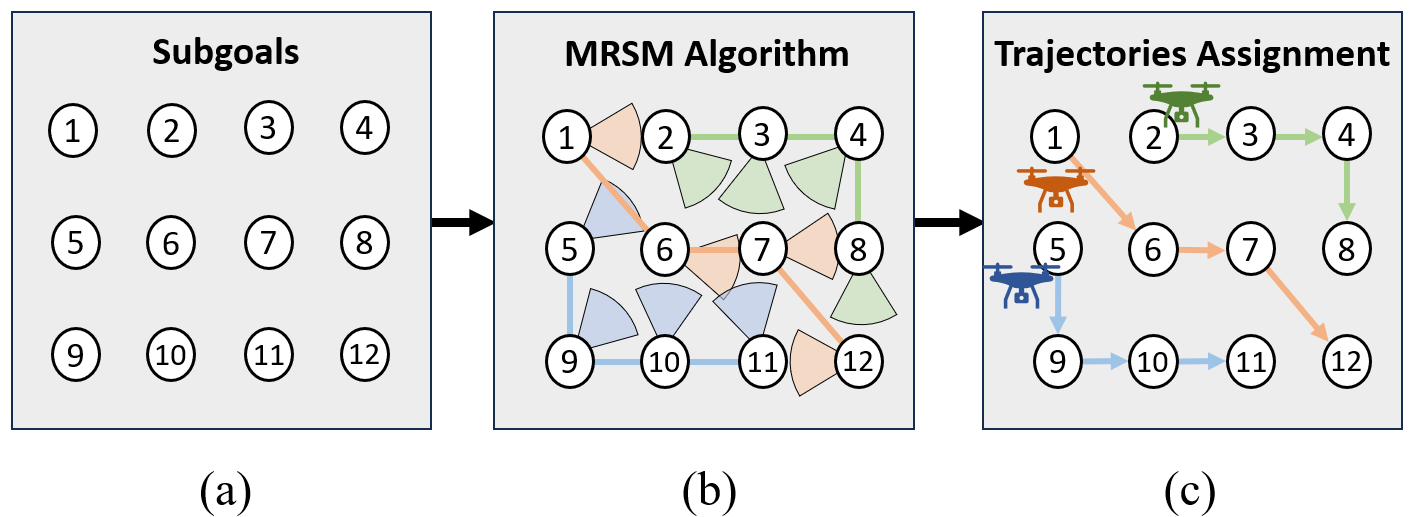
\includegraphics[width=1\textwidth]{overview-2.png}}
\caption{Overview of the proposed multi-robot search system with three robots.
(a) An example of subgoals (nodes) in a search environment.
(b) The trajectories for each robot (orange, blue, and green lines) are obtained by the proposed algorithm (MRSM). The circular sectors are the coverage areas.
(c) The trajectories are assigned to robots to find targets in the environment.
}
\label{overview}
\end{figure}


%\begin{figure}[htbp]
%\centering
%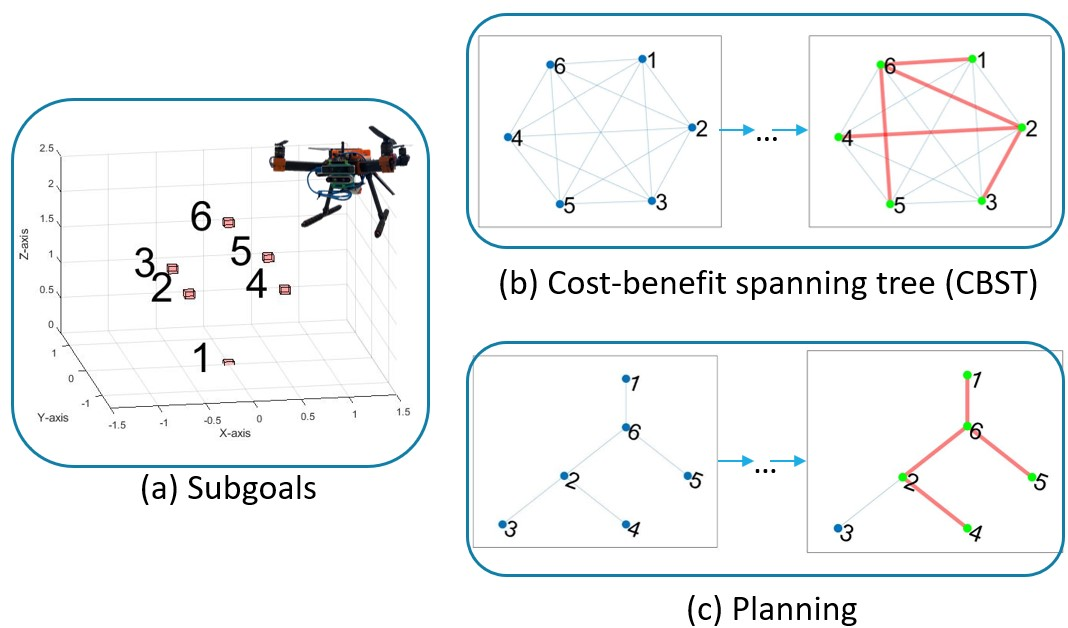
\includegraphics[width=1.0\linewidth]{method_intro.jpg}
%\caption{ Illustration of the proposed method.
%(a) Subgoals.
%The blue points and decimal numbers represent subgoals and the index of subgoals, respectively.
%(b) The cost-benefit spanning tree.
%The green points, red lines and decimal numbers represent nodes in spanning tree, edges in spanning tree and the index of subgoals, respectively.
%(c) Path.
%The green points and red lines represent the path nodes and path edges, respectively.
%}
%%(b) The change of objective function from minimum spanning tree to cost-benefit spanning tree (c) Tree structure of \emph{CBST}.}
%\label{fig:method_intro}
% \end{figure}


For search via learning approaches,
the researchers propose a probability density function (PDF) as a reward function that generates a sequence of decisions based on the reinforcement learning method \cite{sheng2022pd}.
The search problem and the allocation problem are solved by selecting actions with the maximal individual reward function for each robot.
Yet, the graph only considers the unit cost for routing, and the balance of the robots' workloads is not taken into account, potentially resulting in poor task assignment.

To resolve the aforementioned issues, this research proposes a Multi-Robot Search with Matroid constraints (MRSM) algorithm\footnote{The primary distinction between MRSIS and MRSM is that MRSIS models the clustering and routing constraints as independence systems while MRSM models two constraints as matroids.}, which is an improved version of MRSIS algorithm\cite{li2024mrsis}.
Maximal coverage and balanced workloads are considered simultaneously.
The coverage function is to cover a larger area for robots, while the balancing function is to measure the equality of the workloads assigned to robots.
Besides, the routing constraint is reformulated as matroid to boost the theoretical guarantees of the MRSIS \cite{li2024mrsis}.

The proposed MSRM method is illustrated in Fig. \ref{overview}. Given an environment map with subgoals, the goal is to find all targets with multiple robots as soon as possible.
In Fig. \ref{overview}(a), subgoals are evenly distributed in the space. A weighted graph $\mathcal{G}(V,E, w)$ is constructed, where $V$ represents the subgoal set, $E$ represents the edge set, and $w$ is an Euclidean distance function.
In Fig. \ref{overview}(b), the MSRM generates a set of trajectories that maximize the environment coverage and maintain balanced workloads among robots.
In Fig. \ref{overview}(c), trajectories are then assigned to robots to search for targets in the environment.

In this research, some assumptions are made. First, MRSM relies on known environments. A set of subgoals is evenly distributed in the search environments.
Second, the coverage at every subgoal can be pre-computed since the search method is based on known maps.
Third, the perception of robots includes uncertainty and targets may be occluded in the environment.

The contributions of this research are as follows.
First,  the submodular maximization under matroid intersection constraints (MRSM) is proposed for multi-robot search problems.
To the best of our knowledge, this is the first work to propose this objective for these problems.
Second, thanks to the submodularity,
the theoretical guarantees of MRSIS \cite{li2024mrsis} and MRSM are proved as $\frac{1}{2+k_G} \overline{OPT}$ and $\frac{1}{3}\widetilde{OPT}$, respectively, where $k_G > 1$, $\overline{OPT}$ is an approximately optimal solution of the MST or TSP solver and $\widetilde{OPT}$ is an approximately optimal solution of the spanning tree.
Notice that the theoretical bound of MRSM does not depend on the number of robots.
Third, the experiment results show that the proposed method (MRSM) outperforms state-of-the-art approaches (e.g., MRSIS \cite{li2024mrsis}, CapAM \cite{paull2022learning} and PD-FAC \cite{sheng2022pd}) in the multi-robot search problem.

This paper is organized as follows. Section 2 reviews the relevant work on target search methods, multi-robot task allocation, and routing constraints. Section 3 describes the background knowledge of this research. Section 4 introduces the problem formulation. Section 5 describes the search algorithm. Section 6 describes the experiments and analyzes the results. Finally, Section 7 draws conclusions and outlines future work.

\section{Publication Note}
Portions of the literature survey, problem formulation, and experiments appeared in \cite{li2024mrsis}, \cite{li2024casmo}, \cite{li2024mrsm}.


